\vspace{1.5cm}

\subsubsection{Tamaño de los disipadores para cada transistor (resistencia térmica disipador-ambiente)}
\label{thermal_calculation}

Primero determinamos de los puntos de trabajo calculados en la sección~\sectref{qpoint}, las potencias disipadas en cada uno de los transistores de señal y potencia media, los resultados se resumen en el cuadro~\tableref{table:table_powers}


%% \noindent
%% \begin{center}
 
%%\begin{spacing}{1}  
\begin{table}[H]  %%\centering
    
    \setlength\arrayrulewidth{1.5pt}
    \arrayrulecolor{white}
    \def\clinecolor{\hhline{|>{\arrayrulecolor{white}}-%
    >{\arrayrulecolor{white}}|-|-|-|-|-|}}
\resizebox{0.8 \textwidth}{!}{% 
       
\begin{tabularx}{1 \textwidth}%
    {|
    >{\columncolor{white} \centering\arraybackslash}m{0.29\linewidth}
     |
    >{\columncolor{white} \centering\arraybackslash}m{0.14\linewidth}
     |
    >{\columncolor{white} \centering\arraybackslash}m{0.14\linewidth}
     |
    >{\columncolor{white} \centering\arraybackslash}m{0.14\linewidth}
     |
    >{\columncolor{white} \centering\arraybackslash}m{0.14\linewidth}
     |
    >{\columncolor{white} \centering\arraybackslash}m{0.14\linewidth}
     |
    }
    \rowcolor{HeadersColor} \cellcolor{white} \thead{}  & \thead{$Q_{402}$} & \thead{$Q_{403}$} & \thead{$Q_{404}$} & \thead{$Q_{405}$} & \thead{$Q_{406}$} \\
    
    \hhline{|-|-|-|-|-|}
    \rowcolor{gray!20} \cellcolor{gray!40} $I_{C}$ [$\si[per-mode=symbol]{\milli\ampere}$] & $0.54$ & $8.66$ & $9$ & $6$ & $5.5$  \\
    \hhline{|-|-|-|-|-|}
    \rowcolor{gray!20} \cellcolor{gray!40} $V_{CE}$ [$\si[per-mode=symbol]{\volt}$] & $26.1$ & $1.8$ & $27.95$ & $29.4$ & $29.4$  \\
    \hhline{|-|-|-|-|-|}
    \rowcolor{Butter!20} \cellcolor{gray!40}  $P_{D}$ [$\si[per-mode=symbol]{\watt}$] & $14.1 \si[per-mode=symbol]{\milli}$ & $15.6 \si[per-mode=symbol]{\milli}$ & $251 \si[per-mode=symbol]{\milli}$ & $228 \si[per-mode=symbol]{\milli}$ & $228 \si[per-mode=symbol]{\milli}$ \\
    \hhline{|-|-|-|-|-|}
    \rowcolor{gray!20} \cellcolor{gray!40} \thead{\cellcolor{gray!40} \color{black} $P_{D_{max}}^{*}$ [$\si[per-mode=symbol]{\watt}$] } & $625 \si[per-mode=symbol]{\milli}$ & $625 \si[per-mode=symbol]{\milli}$ & $1.25$ & $1.25$ & $1.25$  \\
    \hhline{|-|-|-|-|-|}  
    \rowcolor{gray!20} \cellcolor{gray!40} \thead{\cellcolor{gray!40} \color{black} $\theta_{ja}^{*}$ [$\si[per-mode=symbol]{\celsius\per\watt}$] } & $200$ & $200$ & $100$ & $100$ & $100$  \\
    \hhline{|-|-|-|-|-|}  
    \rowcolor{gray!20} \cellcolor{gray!40} \thead{\cellcolor{gray!40} \color{black} $\theta_{jc}^{*}$ [$\si[per-mode=symbol]{\celsius\per\watt}$] } & $83.3$ & $83.3$ & $10$ & $10$ & $10$  \\
    \hhline{|-|-|-|-|-|}     
       
    \end{tabularx}}
	\caption{\footnotesize{Potencia disipada en los transistores de señal y media potencia.}}
	\label{table:table_powers}
\end{table}
%%\end{spacing}

%% \end{center}

\footnotesize{
$\left(*\right)$ Los datos se tomaron de las correspondientes hojas de datos.
}\\\\


Para todos los transistores que trabajan en \textbf{clase A}, $Q_{402}$, $Q_{403}$ y $Q_{404}$, las potencias disipadas se calcularon simplemente como $V_{CE} \cdot I_{C}$, ya que esto corresponde a la máxima potencia disipada en el transistor, que se da cuando no hay señal en el mismo.\\

Para los transistores $Q_{405}$ y $Q_{406}$, los drivers de los pares compuestos que integran la etapa de salida en \textbf{clase AB}, se hizo las siguientes  suposiciones simplificadoras, que la tensión \mbox{colector-emisor} en los mismos coincide con la de los transistores de salida y que por los mismos circula una corriente que es $\beta$ veces menor que en los transistores de salida, de esta forma la potencia termina siendo $\beta$ veces menor que en estos. De todas formas se trata de unas suposiciones conservadoras.\\

Para los dos transistores de salida, la potencia máxima disipada se calcula como:

\begin{equation}
      P_{C_{max_{Q_{407}}}} = P_{C_{max_{Q_{4088}}}} = \frac{{V_{CC}}^2}{{\pi}^2 \cdot R_{L}} = 11.4 \si[per-mode=symbol]{\watt}
\end{equation}\\

Y se obtiene entonces para los transistores drivers de los pares:

\begin{equation}
P_{C_{max_{Q_{405}}}} = P_{C_{max_{Q_{406}}}} = \frac{P_{C_{max_{Q_{7}}}}}{\beta_{407}} = \frac{11.4 \si[per-mode=symbol]{\watt}}{50} = 228 \si[per-mode=symbol]{\milli\watt}
\end{equation}\\

Para determinar la necesidad de un disipador térmico en cada uno de los transistores, suponemos su operación sin el mismo y planteamos el circuito térmico correspondiente. Para este planteo se necesitan también los siguientes parámetros:

\begin{enumerate}
\item[$\bm{T_{j_{max}}}$] Temperatura máxima de operación de la juntura del transistor ($150 \si[per-mode=symbol]{\celsius}$ para todos los transistores analizados).
\item[$\bm{T_{j_{e}}}$] Temperatura de operación estimada de la juntura del transistor.
\item[$\bm{T_{a}}$] Temperatura ambiente (tomamos $40 \si[per-mode=symbol]{\celsius}$ como un caso de un circuito encerrado en un gabinete).
\item[$\bm{\theta_{ja}}$] Resistencia térmica de la juntura del transistor al ambiente.\\
\end{enumerate}


Entonces solo tenemos una fuente de potencia, $P_{D}$ (modelada por una fuente de corriente) circulando por la resistencia térmica $\theta_{ja}$ (modelada como una resistencia eléctrica), con lo que la temperatura (modelada por tensión) que se desarrolla sobre la juntura se suma a la temperatura ambiente (modelada por una fuente de tensión), con lo que nos queda:


\begin{equation} \label{eq:thermal_ambient}
T_{j_{e}} = P_{D} \cdot \theta_{ja} + T_{a}
\end{equation}\\

Nos queda para cada uno de los transistores de señal y para los drivers de los pares:

\begin{enumerate}
\item[$\bm{Q_{402}}$] $T_{j_{e_{402}}} = 41.2 \si[per-mode=symbol]{\celsius} $ 
\item[$\bm{Q_{403}}$] $T_{j_{e_{403}}} = 41.3 \si[per-mode=symbol]{\celsius} $ 
\item[$\bm{Q_{404}}$] $T_{j_{e_{404}}} = 65.1 \si[per-mode=symbol]{\celsius} $
\item[$\bm{Q_{405}}$] $T_{j_{e_{405}}} = 62.8 \si[per-mode=symbol]{\celsius} $
\item[$\bm{Q_{406}}$] $T_{j_{e_{406}}} = 62.8 \si[per-mode=symbol]{\celsius} $
\item[$\bm{Q_{407}}$] $T_{j_{e_{407}}} = 62.8 \si[per-mode=symbol]{\celsius} $
\item[$\bm{Q_{408}}$] $T_{j_{e_{408}}} = 62.8 \si[per-mode=symbol]{\celsius} $
\end{enumerate}

Podemos ver que ninguno de los transistores supera la máxima temperatura de trabajo, con lo que concluimos que no necesitan disipador térmico.\\

Para los transistores de salida, ambos son el mismo tipo de transistor, obtenemos las resistencias térmicas de la \textbf{figura 7}, \quotemarks{Power Derating} de la hoja de datos del transistor \textbf{TIP41}, apéndice~\sectref{datasheet_TIP41}. Obtenemos:\\

$\theta_{ja_{Q_{407}}} = \theta_{ja_{Q_{408}}} = 60 \si[per-mode=symbol]{\celsius\per\watt}$ y $\bm{\theta_{jc_{Q_{407}}}} = \bm{\theta_{jc_{Q_{408}}}} = 1.9 \si[per-mode=symbol]{\celsius\per\watt} $.\\

Si aplicamos la expresión~\ref{eq:thermal_ambient} nuevamente, obtenemos para ambos transistores de salida:\\

$T_{j_{e_{407}}} = T_{j_{e_{408}}} =  724 \si[per-mode=symbol]{\celsius} $\\

Muy por encima de la temperatura máxima de trabajo para la juntura, con lo que es necesario un disipador térmico. Para calcular la resistencia térmica máxima del disipador que se necesita, se plantea un circuito térmico, pero ahora conteniendo las resistencias térmicas de la juntura al encapsulado, del encapsulado al disipador y del disipador al ambiente, esta última es la que se necesita determinar, en la figura~\figref{fig:fig_thermal_circuit} se muestra el circuito térmico completo.


\begin{figure}[H] %htb
\begin{center}
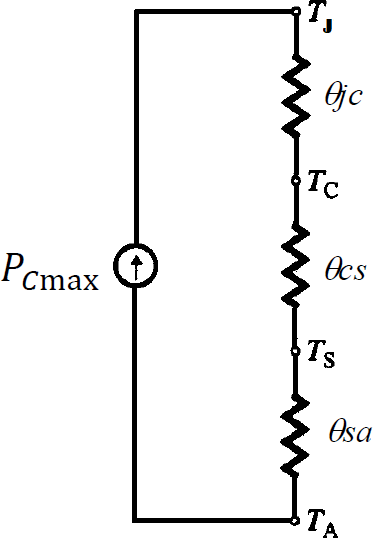
\includegraphics[width=0.35 \textwidth, angle=0]{./img/desarrollo/thermal_circuit.png}
\caption{\label{fig:fig_thermal_circuit}\footnotesize{Circuito térmico para los transistores de salida.}}
\end{center}
\end{figure}

Del planteo de este circuito se despeja la expresión para la resistencia térmica del disipador, $\theta_{sa}$, se obtiene:

\begin{equation}
\theta_{sa} = \frac{T_{J} - T_{a}}{P_{C_{max}}} - \theta_{jc} - \theta_{cs}
\end{equation}


Donde $\theta_{jc}$ ya se obtuvo de las hojas de datos y $\theta_{cs}$, la resistencia térmica del encapsulado al disipador, depende del montaje mecánico que se realiza del transistor sobre el disipador, el mismo puede ser con mica, grasa siliconada, o ambas, el transistor se puede justar mas o menos sobre la superficie del disipador, etc. Teniendo en cuenta estas variantes se estima que $1 \si[per-mode=symbol]{\celsius\per\watt} \leq \theta_{cs} \geq 0.5 \si[per-mode=symbol]{\celsius\per\watt} $, tomamos $1 \si[per-mode=symbol]{\celsius\per\watt}$, el peor caso. Obtenemos entonces para los transistores de salida:

\begin{equation}
\theta_{sa_{max}} = \frac{T_{J} - T_{a}}{P_{C_{max}}} - \theta_{jc} - \theta_{cs} = \frac{150 \si[per-mode=symbol]{\celsius} - 40 \si[per-mode=symbol]{\celsius}   }{11.4  \si[per-mode=symbol]{\watt} } - 1.9 \si[per-mode=symbol]{\celsius\per\watt} - 1 \si[per-mode=symbol]{\celsius\per\watt} \approx 6.8 \si[per-mode=symbol]{\celsius\per\watt}\\ \\
\end{equation}

Con lo que solo necesitamos disipadores para los transistores de salida que cumplan:

\begin{center}
\begin{equation}
\boxed{ \theta_{sa} \leq 6.8 \si[per-mode=symbol]{\celsius\per\watt} }
\end{equation}
\end{center}

\clearpage

\subsubsection{Disipador comercial que podría utilizarse para construir un prototipo funcional}

En la sección anterior calculamos la resistencia térmica que debe tener el disipador térmico de los transistores de salida, se encontró que, $\theta_{sa} \leq 6.8 \si[per-mode=symbol]{\celsius\per\watt}$, usando este valor como referencia se seleccionó un disipador que sería adecuado, el mismo se muestra en la figura~\figref{fig:fig_thermal_dissipator}, tiene $\theta_{sa} = 5.1 \si[per-mode=symbol]{\celsius\per\watt}$, es el modelo \textbf{6225M ZD-5}.

\begin{figure}[H] %htb
\begin{center}
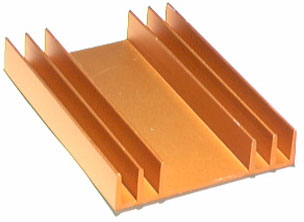
\includegraphics[width=0.6 \textwidth, angle=0]{./img/desarrollo/10b_6225M_ZD_5.png}
\caption{\label{fig:fig_thermal_dissipator}\footnotesize{Disipador térmico seleccionado (\textbf{6225M ZD-5}).}}
\end{center}
\end{figure}


\subsubsection{Comparación con los disipadores utilizados originalmente por Turner}

No pudimos encontrar información acerca del valor de la resistencia térmica de los disipadores usados originalmente, pero de las fotos que hay disponibles, los disipadores eran tipo \textbf{U}, el tamaño y el largo aparente de las aletas hacen parecer que tiene una masa metálica aproximadamente del mismo tamaño, pero no hay mucho mas que podamos decir, salvo que es probable que los disipadores hayan sido sobre-dimensionados al tratarse de un producto comercial, y que probablemente la temperatura interna del gabinete sea superior a la que nosotros consideramos.




\clearpage
